Для начала выведем список доступных сетевых интерфейсов из ARP-кэша при помощи следующей команды:

\begin{verbatim}
$ arp -vn
\end{verbatim}

Результат выполнения команды представлен на рисунке~\ref{ssh_1:ssh_1}.

Из полученной информации можно сделать вывод, что Raspberry Pi имеет IP-адрес в локальной сети 10.42.0.67. Для того, чтобы удаленно подсоединиться к нему по ssh, необходимо выполнить команду: 

\begin{verbatim}
$ ssh pi@10.42.0.67
\end{verbatim}

Далее система запрашивает пароль от Raspberry, после чего устанавливается ssh-соединение (рис.~\ref{ssh_2:ssh_2}).


\begin{figure}[h!]
\center{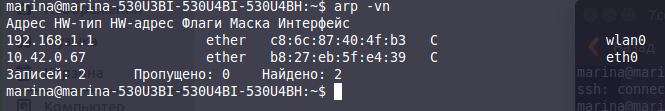
\includegraphics[width=0.8\linewidth]{ssh_1}}
\caption{ Результат выполнения команды arp -vn }
\label{ssh_1:ssh_1}
\end{figure}

\begin{figure}[h!]
\center{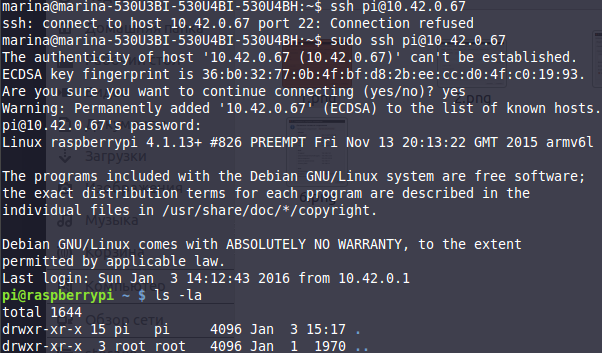
\includegraphics[width=0.8\linewidth]{ssh_2}}
\caption{ Установка ssh-соединения }
\label{ssh_2:ssh_2}
\end{figure}

\clearpage
